\begin{figure}[ht]
	\section{Autores con mayor H-Index y su relación con las tendencias de palabras clave y referencias}
	\centering
	\begin{subfigure}[b]{0.48\textwidth}
		\centering
		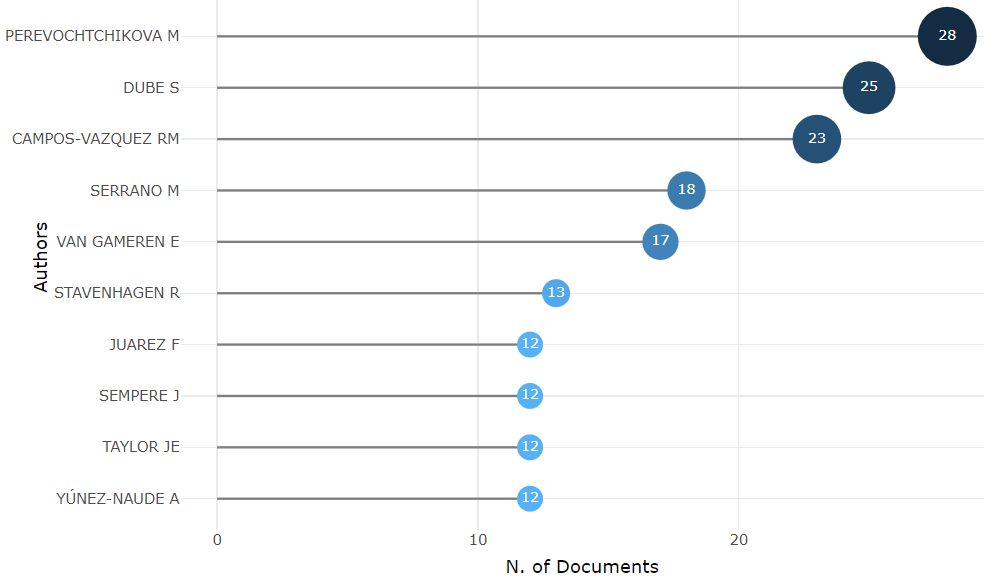
\includegraphics[width=.9\textwidth]{imagenes/au_productivos.png}
		\caption{Autores más productivos}
		\label{fig:au_productivos}   
	\end{subfigure}
	\hfill
	\begin{subfigure}[b]{0.48\textwidth}
		\centering
		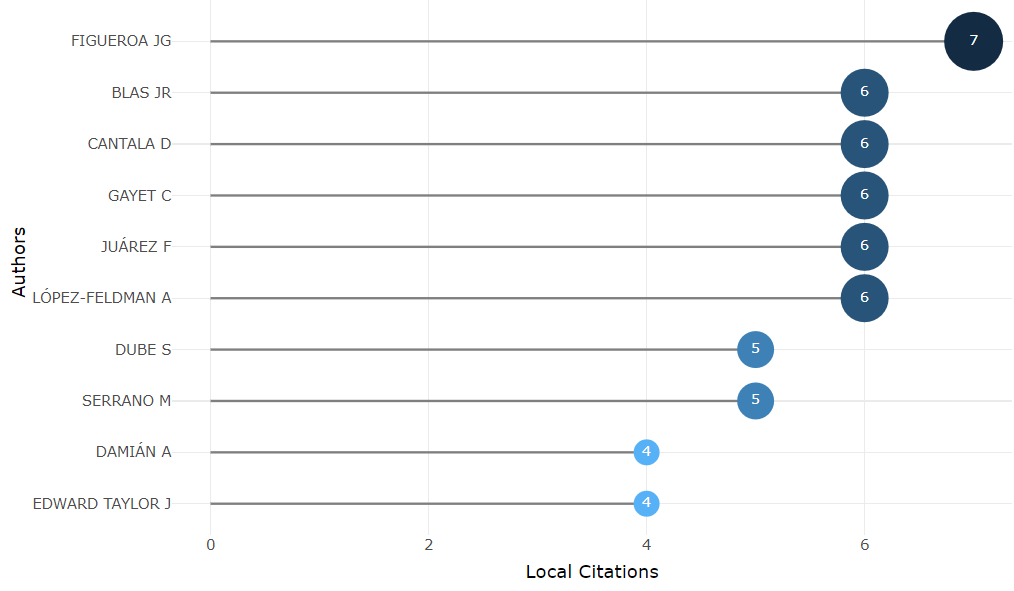
\includegraphics[width=0.9\textwidth]{imagenes/au_citados.png}
		\caption{Autores más citados (dentro del conjunto de datos análizado).}
		\label{fig:au_citados} 
	\end{subfigure}
	\caption{Autores más productivos y más citados.}
	\label{fig:autores} 
\end{figure}

\begin{figure}[ht]
	\centering
	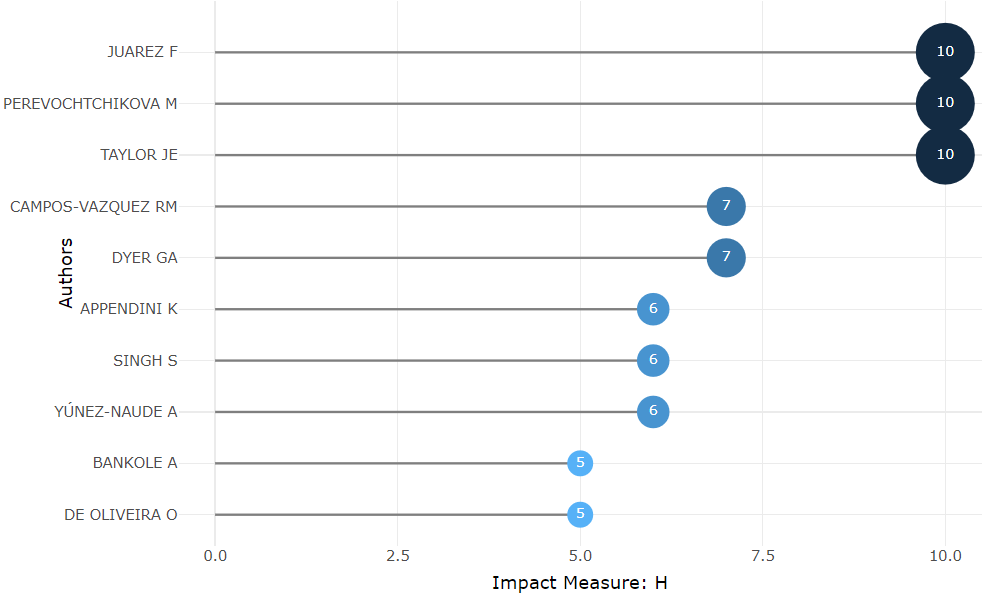
\includegraphics[width=0.8\textwidth]{imagenes/au_hindex.png}
	\caption{Autores con mayor \textit{H-Index} (dentro del conjunto de datos análizado).}
	\label{fig:au_hindex} 
\end{figure}

\begin{figure}[hp]

	\centering
	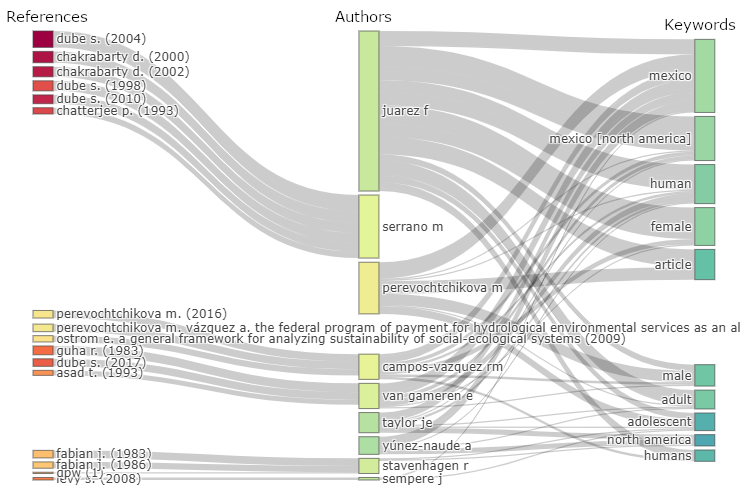
\includegraphics[width=0.8\textwidth]{imagenes/three_field.png}
	\caption{Impacto entre los autores con mayor \textit{H-Index} en las tendencias de referencias y palabras clave.}
	\label{fig:3field} 
\end{figure}

\begin{figure}[ht]
	
	\centering
	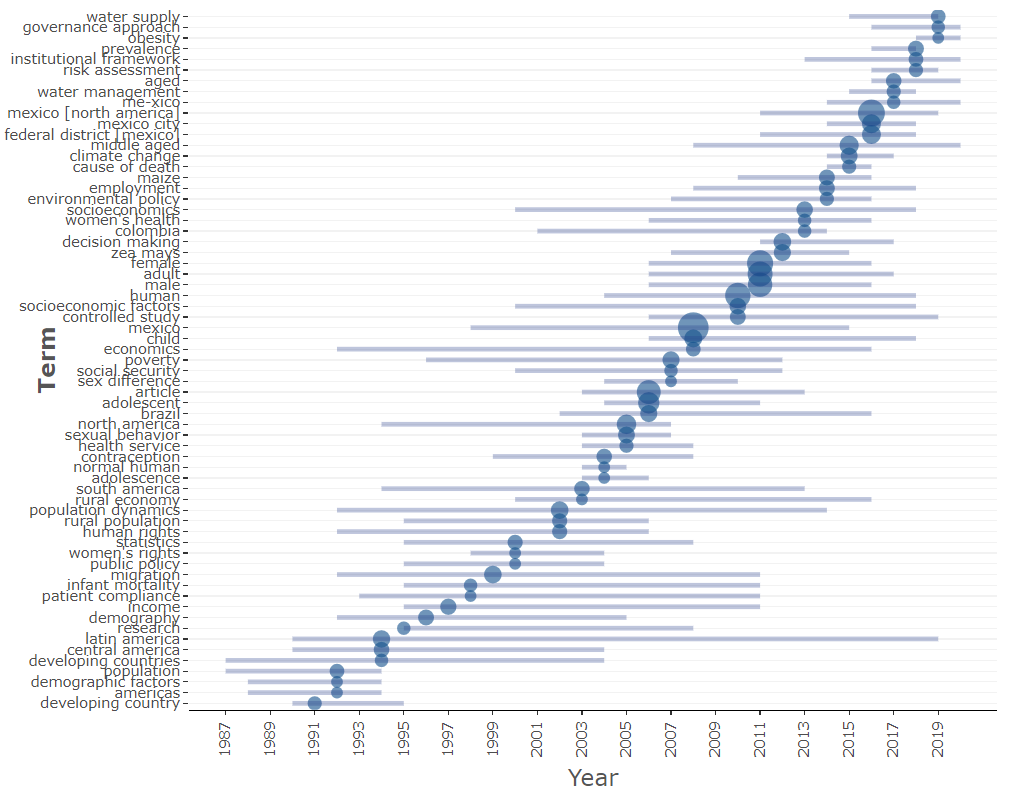
\includegraphics[width=0.8\textwidth]{imagenes/trend_topics.png}
	\caption{Evoluación de las temáticas de investigación con base en las tendencias en palabras clave.}
	\label{fig:trend_topic} 
\end{figure}


